\documentclass[12pt]{article}

\usepackage{sbc-template}

\usepackage{graphicx,url}
\usepackage{subcaption}
\usepackage{float}

\usepackage[brazil]{babel}
\usepackage[utf8]{inputenc}  

%para tabelas mais complexas
\usepackage{tabularx}
\usepackage{booktabs}
\usepackage{caption}
\usepackage{amsmath}

\usepackage[hidelinks]{hyperref}
     
\sloppy

\title{Digitalização da Caderneta da Gestante: Um Ecossistema de IA Responsável para Apoio à Decisão Clínica no Pré-Natal}

\author{Lucas Zegrine Duarte\inst{1}, Humberto Torres Marques Neto\inst{1}}

\address{Instituto de Ciências Exatas e Informática\\
  Pontifícia Universidade Católica de Minas Gerais (PUC Minas)\\
  Caixa Postal 1.686 – 30.535-901 – Belo Horizonte – MG – Brazil
  \email{\{humberto.neto, lucas.duarte\}@sga.pucminas.br}
}

%%%%%%%%%%%%%%%%%%%%%%%%%%%%%%%%%%%%%%%%%%%%%%%%%%%%%%%%%%%%%%%%%%%%%%%%%%%%%%%%%%%%%%%%%%%%%%%%%%%%%%%%%%%%%%%%%%%%%%%%%%%%%%%%%%%%%%%%%%%%%%%%%%%%%%%%%%%%%%%%%%%%%%

\begin{document}

\maketitle

\begin{abstract}
  Prenatal documentation in Brazil is fragmented between physical and digital records, while the use of \textit{Large Language Models} in the public sector poses privacy and hallucination risks.
  This work proposes an \textit{on-premise} architecture integrating local voice transcription (\textit{Faster-Whisper}), \textit{Retrieval-Augmented Generation} over Ministry of Health manuals orchestrated via \textit{Ollama}, and a dedicated privacy gateway to mask PII before model inference.
  To ensure clinical safety, a mandatory human-in-the-loop validation constraint is applied. The primary contribution is a secure and replicable high-fidelity prototype.
  The main limitation is the dependence on local hardware with high \textit{VRAM} capacity to support low-latency inference.
\end{abstract}

\begin{resumo}
  A documentação de pré-natal no Brasil é fragmentação entre registros físicos e digitais e o uso de \textit{Modelos de Linguagem de Grande Escala} no setor público levanta riscos de privacidade e alucinação.
  Este trabalho propõe uma arquitetura \textit{on-premise} que integra transcrição de voz local (\textit{Faster-Whisper}), \textit{Geração Aumentada por Recuperação} sobre manuais do Ministério da Saúde com orquestração via \textit{Ollama} e um gateway de privacidade dedicado para mascarar PII antes da inferência do modelo.
  Para garantir a segurança clínica, aplica-se uma restrição de validação humana obrigatória. A contribuição principal é a materialização de um protótipo de alta fidelidade replicável e seguro.
  A principal limitação é a dependência de hardware local com alta capacidade de \textit{VRAM} para suportar inferências com baixa latência.
\end{resumo}

\noindent \textbf{Palavras-chave:} Cuidado pré-natal; Inteligência artificial; Sistemas de informação em saúde; Privacidade de dados; Geração Aumentada por Recuperação; IA Explicável.

%%%%%%%%%%%%%%%%%%%%%%%%%%%%%%%%%%%%%%%%%%%%%%%%%%%%%%%%%%%%%%%%%%%%%%%%%%%%%%%%%%%%%%%%%%%%%%%%%%%%%%%%%%%%%%%%%%%%%%%%%%%%%%%%%%%%%%%%%%%%%%%%%%%%%%%%%%%%%%%%%%%%%%

\section{Introdução}

A Inteligência Artificial (IA) tem demonstrado potencial transformador na saúde pública, oferecendo soluções para otimização de fluxos de trabalho e suporte à decisão \cite{Rajpurkar2022, Cabitza2022}.
No contexto do atendimento pré-natal, aplicações preditivas baseadas em aprendizado de máquina evidenciam eficácia na identificação precoce de riscos gestacionais \cite{HighRiskPregnancy2025, MachineLearning2022}.
Contudo, a mortalidade e morbidade materna no Brasil permanecem como desafios de saúde pública persistentes, frequentemente agravados por gargalos no acesso e registro adequado de dados durante a assistência \cite{AcessoPreNatal2018, Laurenti2010}.

A documentação clínica no \textit{Sistema Único de Saúde} (SUS) enfrenta um cenário de fragmentação, exigindo que o profissional de saúde registre informações simultaneamente em plataformas digitais pelo e-SUS e em ferramentas físicas, como a Caderneta da Gestante.
Essa dualidade impõe maior carga cognitiva durante as consultas, comprometendo o tempo de contato direto e humanizado com a paciente \cite{ThemeFilha2014, Rajpurkar2022}.

Para atenuar essa sobrecarga, o presente trabalho propõe a especificação de uma plataforma digital \textit{on-premise} que integra transcrição de voz para texto (\textit{Speech-to-Text}) com agentes de Inteligência Artificial baseados em \textit{Geração Aumentada por Recuperação} (RAG) facilitadores de conhecimento de bases de protocolos de cuidado pré-natal.
A ideia principal é automatizar o preenchimento de formulários clínicos durante a consulta, e auxiliar o profissional no cuidado com a paciente utilizando como referências os protocolos oficiais do Ministério da Saúde disponíveis nas cartilhas de estratificação de risco.

%\subsection{Justificativa}
% Justificativa
%  - Depoimentos de profissionais de saúde sobre a solucao proposta e o cenario atual
%  - Deve háver método para coletar depoimentos de profissionais de saúde sobre a solucao proposta e o cenario atual na landing page
%  - Pode levar a necessidade de liberacao de comite de etica

Complicações gestacionais e gravidez de alto risco demandam acompanhamento rigoroso.
Segundo as diretrizes dos Manuais de Gestação de Alto Risco do Ministério da Saúde \cite{ManualAltoRisco2022, ManualAltoRisco2012}, condições de risco ou morbidades pré-existentes exigem uma estratificação contínua e o acesso rápido a protocolos de intervenção específicos, fatores que podem sobrecarregar o tempo de atendimento do profissional e geram impactos expressivos na infraestrutura do sistema público \cite{MaternalMorbidity2025}.

Para otimizar esse monitoramento e atenuar a sobrecarga informacional, modelos generativos têm sido progressivamente propostos como assistentes virtuais clínicos para resumo e triagem de dados \cite{Clusmann2023, Rajpurkar2022}.

No entanto, a implantação irrestrita de Modelos de Linguagem de Grande Escala (LLMs) em cenários públicos depara-se com duas barreiras críticas: o risco de exposição de dados sensíveis (\textit{Personally Identifiable Information} - PII) \cite{OWASPLLM2023, Atheniense2024}, violando normativas como a Lei Geral de Proteção de Dados (LGPD), e a propensão à geração de condutas clínicas fabricadas, as alucinações algorítmicas.

Portanto, a justificativa técnica deste projeto fundamenta-se na necessidade de estruturar uma arquitetura que:
(i) assegure a governança absoluta dos dados por meio de processamento local e isolado;
(ii) minimize o impacto das alucinações utilizando (\textit{RAG}) para ancorar o agente estritamente em protocolos de referência das cartilhas governamentais;
(iii) adote um \textit{gateway} de privacidade dedicado aliado a estratégias de \textit{human-in-the-loop} para assegurar constante supervisão médica \cite{FrameworkGovBR2025};
e (iv) incorpore mecanismos de anonimização e pseudonimização de \textit{PII} antes de submeter informações sensíveis aos modelos generativos.

% Problema de Pesquisa

A pesquisa baseia-se na seguinte pergunta norteadora: \textit{Como especificar e arquitetar um sistema de apoio ao pré-natal que reduza a carga cognitiva do profissional de saúde, garantindo privacidade local de dados (LGPD) e mitigando alucinações sem eximir a validação médica da tomada de decisão?}

Para responder a este problema geral, três subquestões operacionais são investigadas:
\begin{itemize}
  \item Como construir uma topologia de rede isolada em contêineres que impossibilite o vazamento de áudio ou dados textuais sensíveis para a internet pública?
  \item Como mitigar situações em que o profissional confia excessivamente nas sugestões algorítmicas devido à fadiga por meio de um fluxo \textit{human-in-the-loop}?
  \item Como avaliar a qualidade do modelo e da recuperação de informações na ausência de validação inicial em campo por um Comitê de Ética em Pesquisa?
\end{itemize}

% Objetivo Geral

Este projeto possui como objetivo geral especificar e arquitetar uma plataforma digital \textit{on-premise} para apoio ao pré-natal, integrando \textit{LLMs} fundamentada via \textit{RAG} para reduzir a carga cognitiva do atendimento, com foco em explicabilidade, privacidade e alinhamento às diretrizes da LGPD.

% Objetivos Específicos

Para atingir o objetivo geral, delineiam-se os seguintes objetivos específicos:

\begin{enumerate}
  \item Revisar a literatura sobre IA Responsável em saúde pública, focando em explicabilidade, privacidade e governança de dados no contexto do SUS;
  \item Formalizar os requisitos técnicos e as histórias de usuário, mapeando a interação entre profissionais de saúde e o sistema para o suporte ao cuidado gestacional;
  \item Projetar uma topologia de implantação on-premise replicável via contêineres (\textit{Docker}), garantindo a soberania dos dados.
  \item Projetar e descrever o fluxo de dados integrando transcrição (\textit{STT}), um \textit{gateway} de privacidade dedicado para mascaramento de PII e recuperação de conhecimento (\textit{RAG}).
  \item Definir mecanismos de mitigação contra alucinações e ameaças de \textit{prompt injection}, estabelecendo protocolos de anonimização e revisão humana obrigatória.
\end{enumerate}

Para viabilizar este escopo, a pesquisa baseia-se na engenharia de software e no desenvolvimento ágil, validando os requisitos por meio de casos clínicos sintéticos.
Os resultados obtidos demonstram a efetividade da arquitetura através de um protótipo funcional de alta fidelidade capaz de processar transcrições locais, anonimizar informações e recuperar diretrizes via \textit{RAG} de maneira segura.
O restante deste artigo está estruturado da seguinte forma: apresentação do referencial teórico, seguida pelos materiais, metodologia, solução arquitetural proposta, enquanto as Seções subsequentes reúnem a implementação técnica, a análise dos resultados, a discussão dos achados e, por fim, as conclusões.

%%%%%%%%%%%%%%%%%%%%%%%%%%%%%%%%%%%%%%%%%%%%%%%%%%%%%%%%%%%%%%%%%%%%%%%%%%%%%%%%%%%%%%%%%%%%%%%%%%%%%%%%%%%%%%%%%%%%%%%%%%%%%%%%%%%%%%%%%%%%%%%%%%%%%%%%%%%%%%%%%%%%%%


\section{Referencial Teórico}
% 5. Fundamentacao Teorica
%     - Melhorar coesao entre os artigos
%    5.1 IA em Saúde pública e copilotos clínicos
%    5.2 RAG e ancoragem em diretrizes
%    5.3 Privacidade: LGPD, minimizacao, processamento on-premise
%    5.4 Human-in-the-loop e responsabilidade clinica
%    5.5 MCP e Tooling para governanca de contexto
%    5.6 Security by design no desenvolvimento de agentes de IA (OWASP top 10 for llm applications)
%    5.7 Caso de Uso dda Micorosoft com o Presidio como referencia comparativa (mitigação de Sensitive Data Exposure e Indirect Prompt Injection através do uso do Microsoft Presidio) (NER customizado para PII)
%    5.8 Trabalhos correlatos (comparar com 2 projetos similares) (validar lacuna de projetos no contexto atual) (tabela comparativa com 2 projetos similares)
% deve apresentar o que sao as tenicas propostas a serem utilizadas e como elas serão aplicadas a partir de referencial terorico real
%<Paragrafo de introducao>

\subsection{IA Responsável e Governança em Saúde}
A IA Responsável (RAI) transcende a ética teórica ao propor a operacionalização de princípios de transparência e justiça na engenharia de software \cite{Shneiderman2021, Dignum2022}. Na saúde, essa necessidade é suprida por frameworks como o \textit{FUTURE-AI}, que estabelece diretrizes para a implantação de sistemas confiáveis \cite{Lekadir2023}, e o \textit{FAIR-AI}, focado na revisão contínua de modelos clínicos \cite{Lekadir2022}.

No cenário brasileiro, a governança deve alinhar-se à Lei Geral de Proteção de Dados (LGPD) e a frameworks institucionais que buscam mitigar riscos regulatórios e fragmentações normativas no setor público \cite{Atheniense2024, FrameworkGovBR2025}.

\subsection{LLMs e RAG na Saúde Pública}
Modelos de Linguagem de Grande Escala (LLMs) oferecem novas possibilidades para a análise de prontuários. Contudo, devido ao risco de alucinações em contextos clínicos, a técnica de \textit{Retrieval-Augmented Generation} (RAG) é empregada para restringir a base de conhecimento do modelo aos Manuais Técnicos de Pré-Natal do Ministério da Saúde.

%%%%%%%%%%%%%%%%%%%%%%%%%%%%%%%%%%%%%%%%%%%%%%%%%%%%%%%%%%%%%%%%%%%%%%%%%%%%%%%%%%%%%%%%%%%%%%%%%%%%%%%%%%%%%%%%%%%%%%%%%%%%%%%%%%%%%%%%%%%%%%%%%%%%%%%%%%%%%%%%%%%%%%

\section{Materiais}

Nesta seção, são detalhados os componentes que estruturam o sistema, incluindo os requisitos de \textit{hardware} para execução local, os \textit{frameworks} de desenvolvimento, as bases de dados utilizadas e as ferramentas de Inteligência Artificial implementadas.

\subsection{Hardware}
Para viabilizar a arquitetura \textit{on-premise}, o hardware foi dimensionado para atender aos requisitos de inferência do \textit{LLM} clínico.

\begin{table}[H]
  \centering
  \caption{Especificações do hardware utilizado.}
  \label{tab:hardware_specs}
  \small
  \begin{tabularx}{\textwidth}{l X}
    \toprule
    \textbf{Componente} & \textbf{Especificação}           \\
    \midrule
    CPU                 & Intel Core i7-14700K             \\
    GPU                 & Nvidia RTX 5060 Ti 16GB          \\
    RAM                 & Vengeance 2x 16GB DDR5 6000MHz   \\
    PSU                 & 750W Gold Corsair                \\
    Motherboard         & Asus ROG Strix Z790 Maximus Hero \\
    \bottomrule
  \end{tabularx}
\end{table}

O poder computacional mínimo depende primariamente da quantidade de VRAM dedicada para alocar simultaneamente o motor RAG e os modelos de agente \textit{LLM} clínico.

\subsection{Software e Frameworks}

O ambiente adota \textit{TypeScript} como linguagem principal.
O \textit{backend} foi desenvolvido em \textit{Node.js} utilizando o micro-\textit{framework} Hono para orquestração assíncrona da API.
O \textit{frontend} foi estruturado em React, empregando Vite e TailwindCSS.
A virtualização e o isolamento dos serviços (\textit{sandboxing}) são garantidos pelo uso de contêineres \textit{Docker} de modo a vetar execução de código arbitrário provenientes da orquestração de \textit{LLMs}.

\subsection{Base de Dados}

Para a sustentação transacional de cadastros e triagens, adotou-se o banco relacional PostgreSQL, gerenciado por meio do Prisma ORM.
Como corpo de conhecimento documental, as Cartilhas de Atenção Pré-Natal do Ministério da Saúde foram vetorizadas e processadas como fonte de verdade (\textit{ground truth}) para os agentes, com os documentos listados na Tabela~\ref{tab:cartilhas_sus}.

% \begin{table}[H]
%     \centering
%     \caption{Manuais e cartilhas governamentais utilizadas como base de conhecimento.}
%     \label{tab:cartilhas_sus}
%     \small
%     \begin{tabularx}{\textwidth}{X c c}
%         \toprule
%         \textbf{Título do Documento} & \textbf{Ano} & \textbf{Referência} \\ 
%         \midrule
%         Caderneta da Gestante & 2024 & \cite{CadernetaGestante2024} \\
%         Ficha Pré-natal: Acolhimento e Identificação & 2018 & \cite{FichaPreNatal2018} \\
%         Guia do Pré-natal do Parceiro para Profissionais de Saúde & 2025 & \cite{GuiaPreNatalParceiro2025} \\
%         Cadernos de Atenção Básica: Atenção ao Pré-natal de Baixo Risco & 2012 & \cite{CadernosAtencaoBasica32} \\
%         Atualização em Pré-natal para Profissionais da Atenção Básica & 2014 & \cite{AtualizacaoPreNatalSC2014} \\
%         Guia de Atenção à Saúde: Estratificação de Risco & 2024 & \cite{GuiaAtencaoGestanteMG2024} \\
%         Manual de Gestação de Alto Risco & 2022 & \cite{ManualAltoRisco2022} \\
%         Manual Técnico Gestação de Alto Risco (5ª Ed.) & 2012 & \cite{ManualAltoRisco2012} \\
%         Gestação de Alto Risco: Manual Técnico (5ª Ed.) & 2010 & \cite{ManualAltoRisco2010} \\
%         \bottomrule
%     \end{tabularx}
% \end{table}

\begin{table}[H]
  \centering
  \caption{Base de conhecimento documental: Manuais e cartilhas.}
  \label{tab:cartilhas_sus}
  \small
  % \begin{tabularx}{\textwidth}{X c l}
  \begin{tabularx}{\textwidth}{>{\hsize=1.5\hsize}X c >{\hsize=0.5\hsize}X}
    \toprule
        \textbf{Título do Documento} & \textbf{Ano} & \textbf{Referência} \\ 
    \midrule
        Caderneta da Gestante                                          & 2024 & \cite{CadernetaGestante2024} \\
        Ficha Pré-natal: Acolhimento e Identificação                   & 2018 & \cite{FichaPreNatal2018} \\
        Guia do Pré-natal do Parceiro para Profissionais de Saúde      & 2025 & \cite{GuiaPreNatalParceiro2025} \\
        Cadernos de Atenção Básica: Pré-natal de Baixo Risco           & 2012 & \cite{CadernosAtencaoBasica32} \\
        Guia de Atenção à Saúde: Estratificação de Risco               & 2024 & \cite{GuiaAtencaoGestanteMG2024} \\
        Atualização em Pré-natal para Profissionais da Atenção Básica  & 2014 & \cite{AtualizacaoPreNatalSC2014} \\
        Manual de Gestação de Alto Risco                               & 2022 & \cite{ManualAltoRisco2022} \\
        Manual Técnico Gestação de Alto Risco (5ª Ed.)                 & 2012 & \cite{ManualAltoRisco2012} \\
        Gestação de Alto Risco: Manual Técnico (5ª Ed.)                & 2010 & \cite{ManualAltoRisco2010} \\
    \bottomrule
  \end{tabularx}
\end{table}

\subsection{Ferramentas de IA}

O sistema integra o \textit{Faster-Whisper} para transcrição local e persistência de \textit{embeddings} e metadados de fragmentos de documentos em \textit{SQLite} (serviço \texttt{clinical-ai}), substituindo um armazenamento vetorial dedicado externo.
O dimensionamento deste modelo, focado em 16.384 \textit{tokens} de contexto, demonstrou o melhor custo-benefício frente às limitações de VRAM (Tabela~\ref{tab:latency_compatibility}), cujas flutuações dependem diretamente da arquitetura de \textit{hardware} e de otimizações de \textit{drivers} locais \cite{VRAMCalculator}.

\begin{table}[H]
  \centering
  \caption{Estimativa teórica de consumo de VRAM.}
  \label{tab:latency_compatibility}
  \small
  \begin{tabular}{l c c r}
    \toprule
    \textbf{Modelo}       & \textbf{Contexto} & \textbf{Parâmetros} & \textbf{VRAM}        \\
    \midrule
    GPT-OSS (Q4)          & 16.384            & 20B                 & $\sim$17 GB          \\
    Qwen3.6 (Q4)          & 16.384            & 35B                 & $\sim$24 GB          \\
    Qwen3.5 (Q4)          & 16.384            & 27B                 & $\sim$27 GB          \\
    \textbf{Qwen3.5 (Q4)} & \textbf{16.384}   & \textbf{9B}         & \textbf{$\sim$10 GB} \\
    Qwen3 (Q4)            & 16.384            & 7B                  & $\sim$5 GB           \\
    \bottomrule
  \end{tabular}
\end{table}

A inferência é orquestrada pelo \textit{Ollama} com o modelo Qwen3.5 (9B, quantização Q4), parametrizado para mitigar alucinações (Tabela~\ref{tab:hyperparams}) na arquitetura de hardware disponível.
A estruturação da base de conhecimento inclui o particionamento semântico (\textit{chunking}) das diretrizes e sua vetorização única, com persistência no armazenamento vetorial.
Para gerenciar possíveis sobreposições ou conflitos temporais entre manuais de anos distintos, incorporou-se a técnica de \textit{Maximal Marginal Relevance} (MMR) como mecanismo de re-ranqueamento (\textit{reranking}).
O MMR foi utilizado para descartar redundâncias, filtrando os documentos para reter um subconjunto de contextos que maximiza tanto a relevância em relação à consulta quanto a diversidade informacional apresentada ao modelo.

\begin{table}[H]
  \centering
  \caption{Hiperparâmetros de inferência (Ollama) e RAG.}
  \label{tab:hyperparams}
  \small
  \begin{tabularx}{\textwidth}{l r | l r}
    \toprule
    \multicolumn{2}{c}{\textbf{LLM (Qwen3.5)}} & \multicolumn{2}{c}{\textbf{RAG \& Chunking}}                                                 \\
    \midrule
    \texttt{num\_ctx}                          & 16.384                                       & \texttt{embedding\_model}  & nomic-embed-text \\
    \texttt{num\_batch}                        & 256                                          & \texttt{chunk\_max\_chars} & 900              \\
    \texttt{temperature}                       & 0.1                                          & \texttt{max\_chunks}       & 6                \\
    \texttt{top\_p}                            & 0.9                                          & \texttt{rerank\_enabled}   & True             \\
    \bottomrule
  \end{tabularx}
\end{table}

%%%%%%%%%%%%%%%%%%%%%%%%%%%%%%%%%%%%%%%%%%%%%%%%%%%%%%%%%%%%%%%%%%%%%%%%%%%%%%%%%%%%%%%%%%%%%%%%%%%%%%%%%%%%%%%%%%%%%%%%%%%%%%%%%%%%%%%%%%%%%%%%%%%%%%%%%%%%%%%%%%%%%%

\section{Metodologia}

A pesquisa adota uma abordagem de Engenharia de Software baseada desenvolvimento ágil de software com desenvolvimento dividido em:
(i) Modelagem de dados relacionais para prontuários;
(ii) Desenvolvimento de um webapp para CRM das gestantes por parte do profissional de saúde;
(iii) Implementação de agente "Escriba"  para transcrição de consultas e autopreenchimento do prontuário eletrônico da paciente;
(iv) Desenvolvimento de motor RAG para consulta de protocolos;
(v) Desenvolvimento de um agente de IA para suporte clínico em tempo real;
% (vi) Automação de eventos para mensageria via WhatsApp.

% Coleta, Preparação e Governança de Dados}

Quanto a preparação dos dados, o banco de dados vetorial é alimentado através do \textit{Semantic Chunking} das cartilhas governamentais, garantindo que algoritmos de extração vetorial preservassem a semântica das tabelas de exames pré-natais.
A governança foi configurada em modo \textit{zero-trust}, onde os áudios capturados não são armazenados, e a transcrição \textit{STT} cruza um \textit{gateway} de privacidade que aplica regras para mascaramento de \textit{PII} brasileiras (CPF, CNS, e-mail, telefone e cadeias longas de dígitos) antes de tocar o orquestrador \textit{RAG}.

%adicioanr imagem do fluxo de dados e anonimizacao dos mesmos

% Arquitetura do sistema

A pesquisa adota uma abordagem de Engenharia de Software baseada no desenvolvimento ágil de software com sprints no modelo scrum, contendo:

\begin{itemize}
  \item Revisão Literária e Modelagem de Dados
  \item Desenvolvimento do \textit{Backend} e APIs
  \item Desenvolvimento do \textit{Frontend} (WebApp)
  \item Desenvolvimento do Agente STT via \textit{Whisper} com Diarização
  \item Desenvolvimento do Motor de \textit{RAG} e do \textit{gateway} de privacidade (sidecar de sanitização HTTP)
  \item Desenvolvimento do Agente de IA\@: Assistente Clínico Local
  \item Desenvolvimento do Anonimizador, \textit{Sandboxing} e \textit{Guardrails}
  \item Testes de Carga e Validação
  \item Redação do Artigo Final
\end{itemize}

A arquitetura docker desenhada reflete o isolamento total dos módulos do sistema, sendo esta estratificada em três subredes \textit{Docker} (\texttt{frontend-nw}, \texttt{backend-nw} e \texttt{data-nw}) para cumprir com o objetivo específico de replicabilidade.
Para cumprir com a restrição \textit{Human-in-the-Loop} todo preenchimento de documentos pela IA é impossibilitado e aguarda validação explícita do profissional de saúde.

\begin{figure}[H]
  \centering
  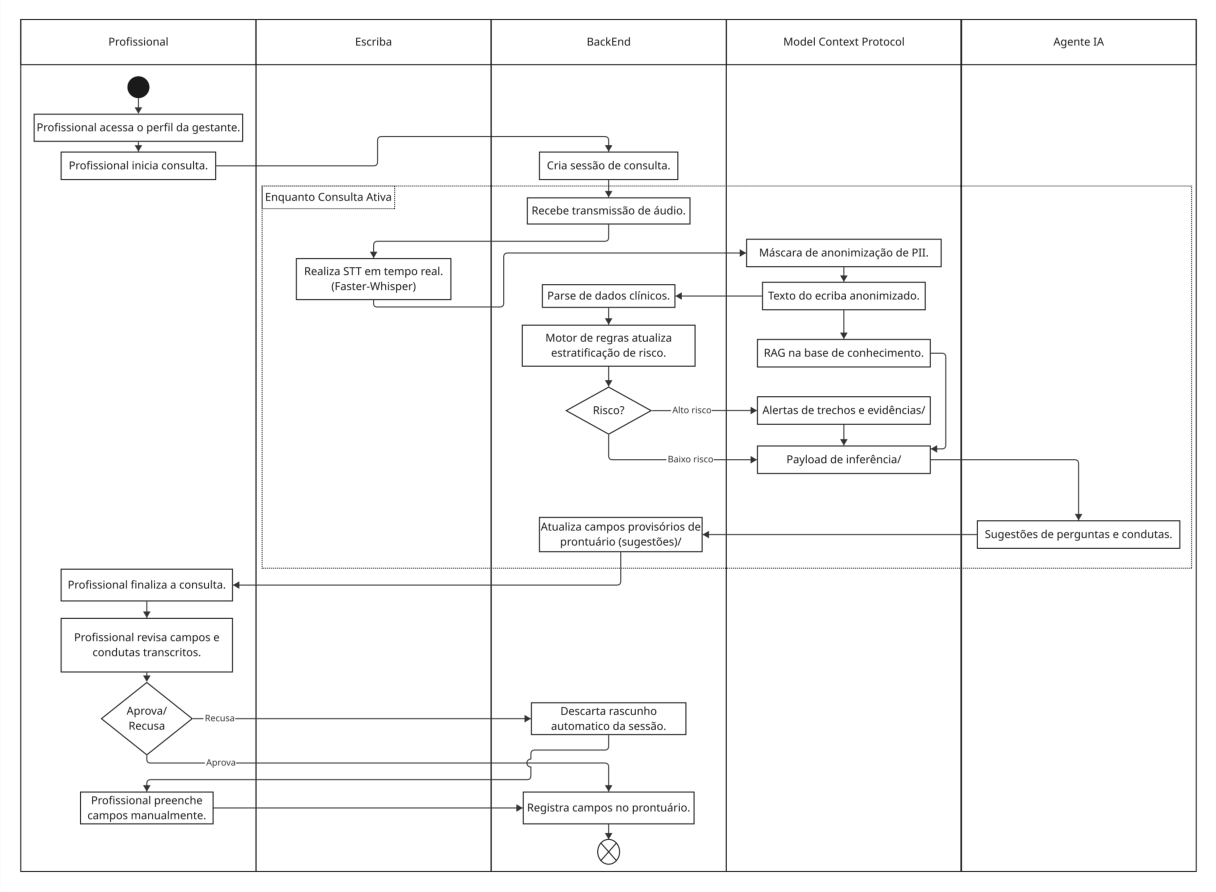
\includegraphics[width=\textwidth, keepaspectratio]{assets/FluxoDeConsulta.pdf}
  \caption{Pipeline arquitetural e ciclo de vida da transação da consulta médica.}
  \label{fig:fluxo_consulta}
\end{figure}

A Figura~\ref{fig:der} ilustra o Diagrama de Entidade-Relacionamento (DER) do esquema de banco de dados normalizado.
A modelagem das entidades, atributos e relacionamentos foi elaborada com base na 8ª edição revisada da \textit{Caderneta da Gestante} do Ministério da Saúde, utilizada como referência para determinar os campos clínicos, administrativos e de acompanhamento presentes no sistema \cite{CadernetaGestante2024}.
Dessa forma, o banco de dados espelha os fluxos da caderneta física e preserva a lógica documental prevista para o acompanhamento pré-natal.

\begin{figure}[H]
  \centering
  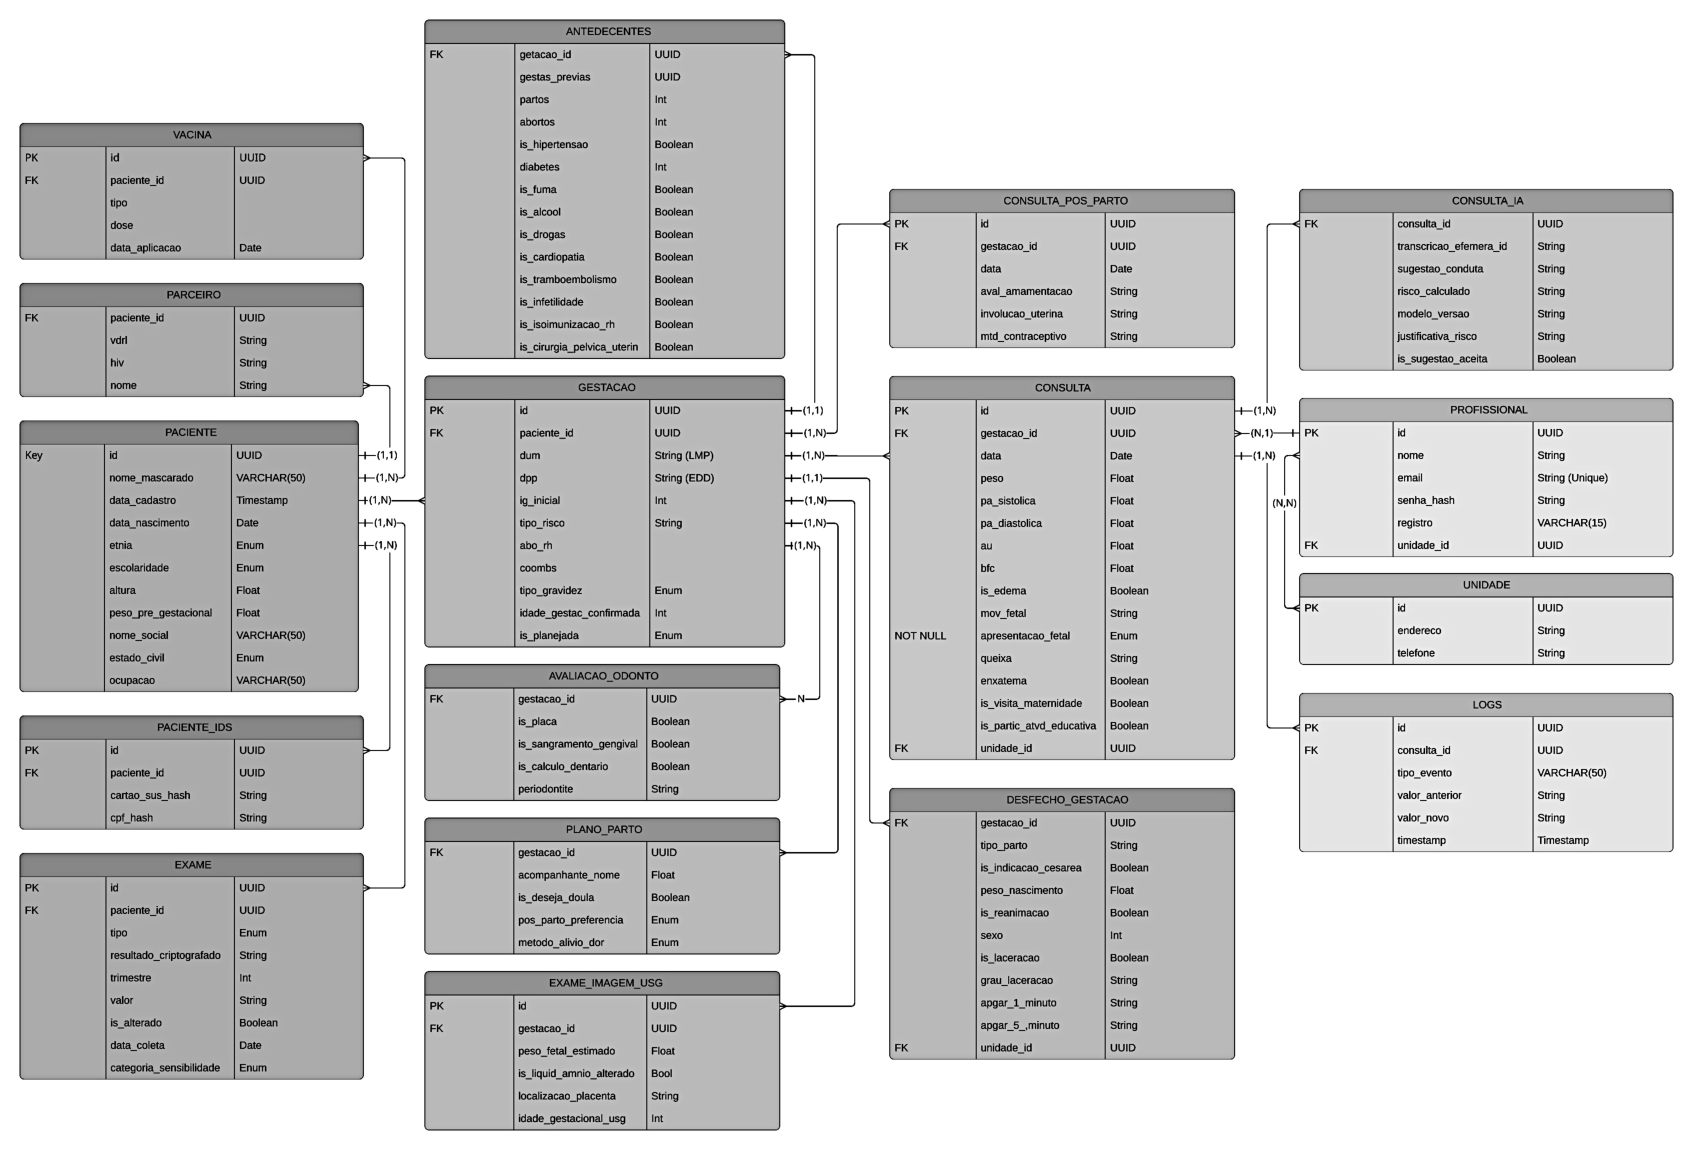
\includegraphics[width=\textwidth, keepaspectratio]{assets/DER_bw.pdf}
  \caption{Diagrama de Entidade-Relacionamento (DER) do sistema.}
  \label{fig:der}
\end{figure}



%%%%%%%%%%%%%%%%%%%%%%%%%%%%%%%%%%%%%%%%%%%%%%%%%%%%%%%%%%%%%%%%%%%%%%%%%%%%%%%%%%%%%%%%%%%%%%%%%%%%%%%%%%%%%%%%%%%%%%%%%%%%%%%%%%%%%%%%%%%%%%%%%%%%%%%%%%%%%%%%%%%%%%

\section{Solução Proposta}

A materialização do ecossistema foi guiada por requisitos funcionais (RF) e histórias de usuário (US) estritos, formalizados para mitigar os riscos inerentes à aplicação clínica de Inteligência Artificial. Dentre os requisitos notáveis que moldaram a proposição da arquitetura, destacam-se:

\begin{itemize}
  \item \textbf{Agente Escriba e Transitoriedade (RF03/RF04):} Exigência de transcrição de voz local em tempo real para preenchimento estruturado de formulários, operando sob a premissa estrita de \textit{não persistir} o áudio bruto ou as transcrições literais nos bancos de dados transacionais.
  \item \textbf{Apoio à Decisão via RAG (RF05):} Implementação de um assistente interativo ancorado de forma exclusiva nos Manuais Técnicos do Ministério da Saúde, bloqueando o fornecimento de condutas baseadas apenas no conhecimento paramétrico generalista do modelo.
  \item \textbf{Validação Obrigatória (\textit{Human-in-the-Loop} - US04):} Restrição sistêmica que impede a consolidação autônoma de qualquer inferência da IA no prontuário definitivo, transferindo a responsabilidade da "aprovação" ou "rejeição" das sugestões obrigatoriamente para o profissional de saúde.
  \item \textbf{Intervenção Manual Corretiva (US07):} Garantia estrutural de que todos os formulários pré-preenchidos pelos agentes generativos sejam plenamente editáveis durante a consulta, prevenindo a persistência de falsos positivos sistêmicos.
  \item \textbf{Mascaramento de PII (US13):} Interceptação e anonimização de dados de identificação pessoal por meio de um \textit{gateway} de privacidade dedicado baseado em padrões brasileiros (CPF, CNS, e-mail, telefone), garantindo conformidade com a LGPD antes de submeter os contextos à inferência semântica.
  \item \textbf{Alertas Sistêmicos de Alto Risco (US05):} Geração automática de sinalizações visuais críticas caso os parâmetros vitais ou laboratoriais extraídos pela IA ultrapassem os limiares de segurança definidos nas cartilhas governamentais.
  \item \textbf{Portabilidade Documental (US06):} Capacidade de exportação dinâmica de todos os registros clínicos em um arquivo PDF espelhado visualmente à ficha oficial de acompanhamento do SUS, assegurando a continuidade do cuidado analógico.
  \item \textbf{Integração Preventiva da Paciente (US10/US11):} Disparo assíncrono de resumos do plano de cuidado e alertas de agendamento via canais de mensageria, visando combater ativamente os índices de evasão nas consultas de acompanhamento.
\end{itemize}

A partir dessas restrições arquiteturais e histórias de usuário, os resultados práticos culminaram em um protótipo funcional de alta fidelidade.
Este artefato traduz o fluxo operacional sob a ótica da usabilidade, visando minimizar a curva de aprendizado e a sobrecarga informacional dos profissionais no SUS.

A Figura~\ref{fig:interfaces_compostas} ilustra o ecossistema proposto em três visões principais:
o painel de gestão de agenda (Figura~\ref{fig:sub_dashboard}),
o perfil consolidado para estratificação de risco da gestante (Figura~\ref{fig:sub_paciente}),
e a interface de consulta em andamento (Figura~\ref{fig:sub_escriba}), ambiente em que o agente Escriba atua na transcrição em tempo real e o agente de \textit{IA} fornece o apoio à decisão clínica.

\begin{figure}[H]
  \centering
  % --- Primeira Subfigura (Antiga Fig 3) ---
  \begin{subfigure}[b]{0.48\textwidth}
    \centering
    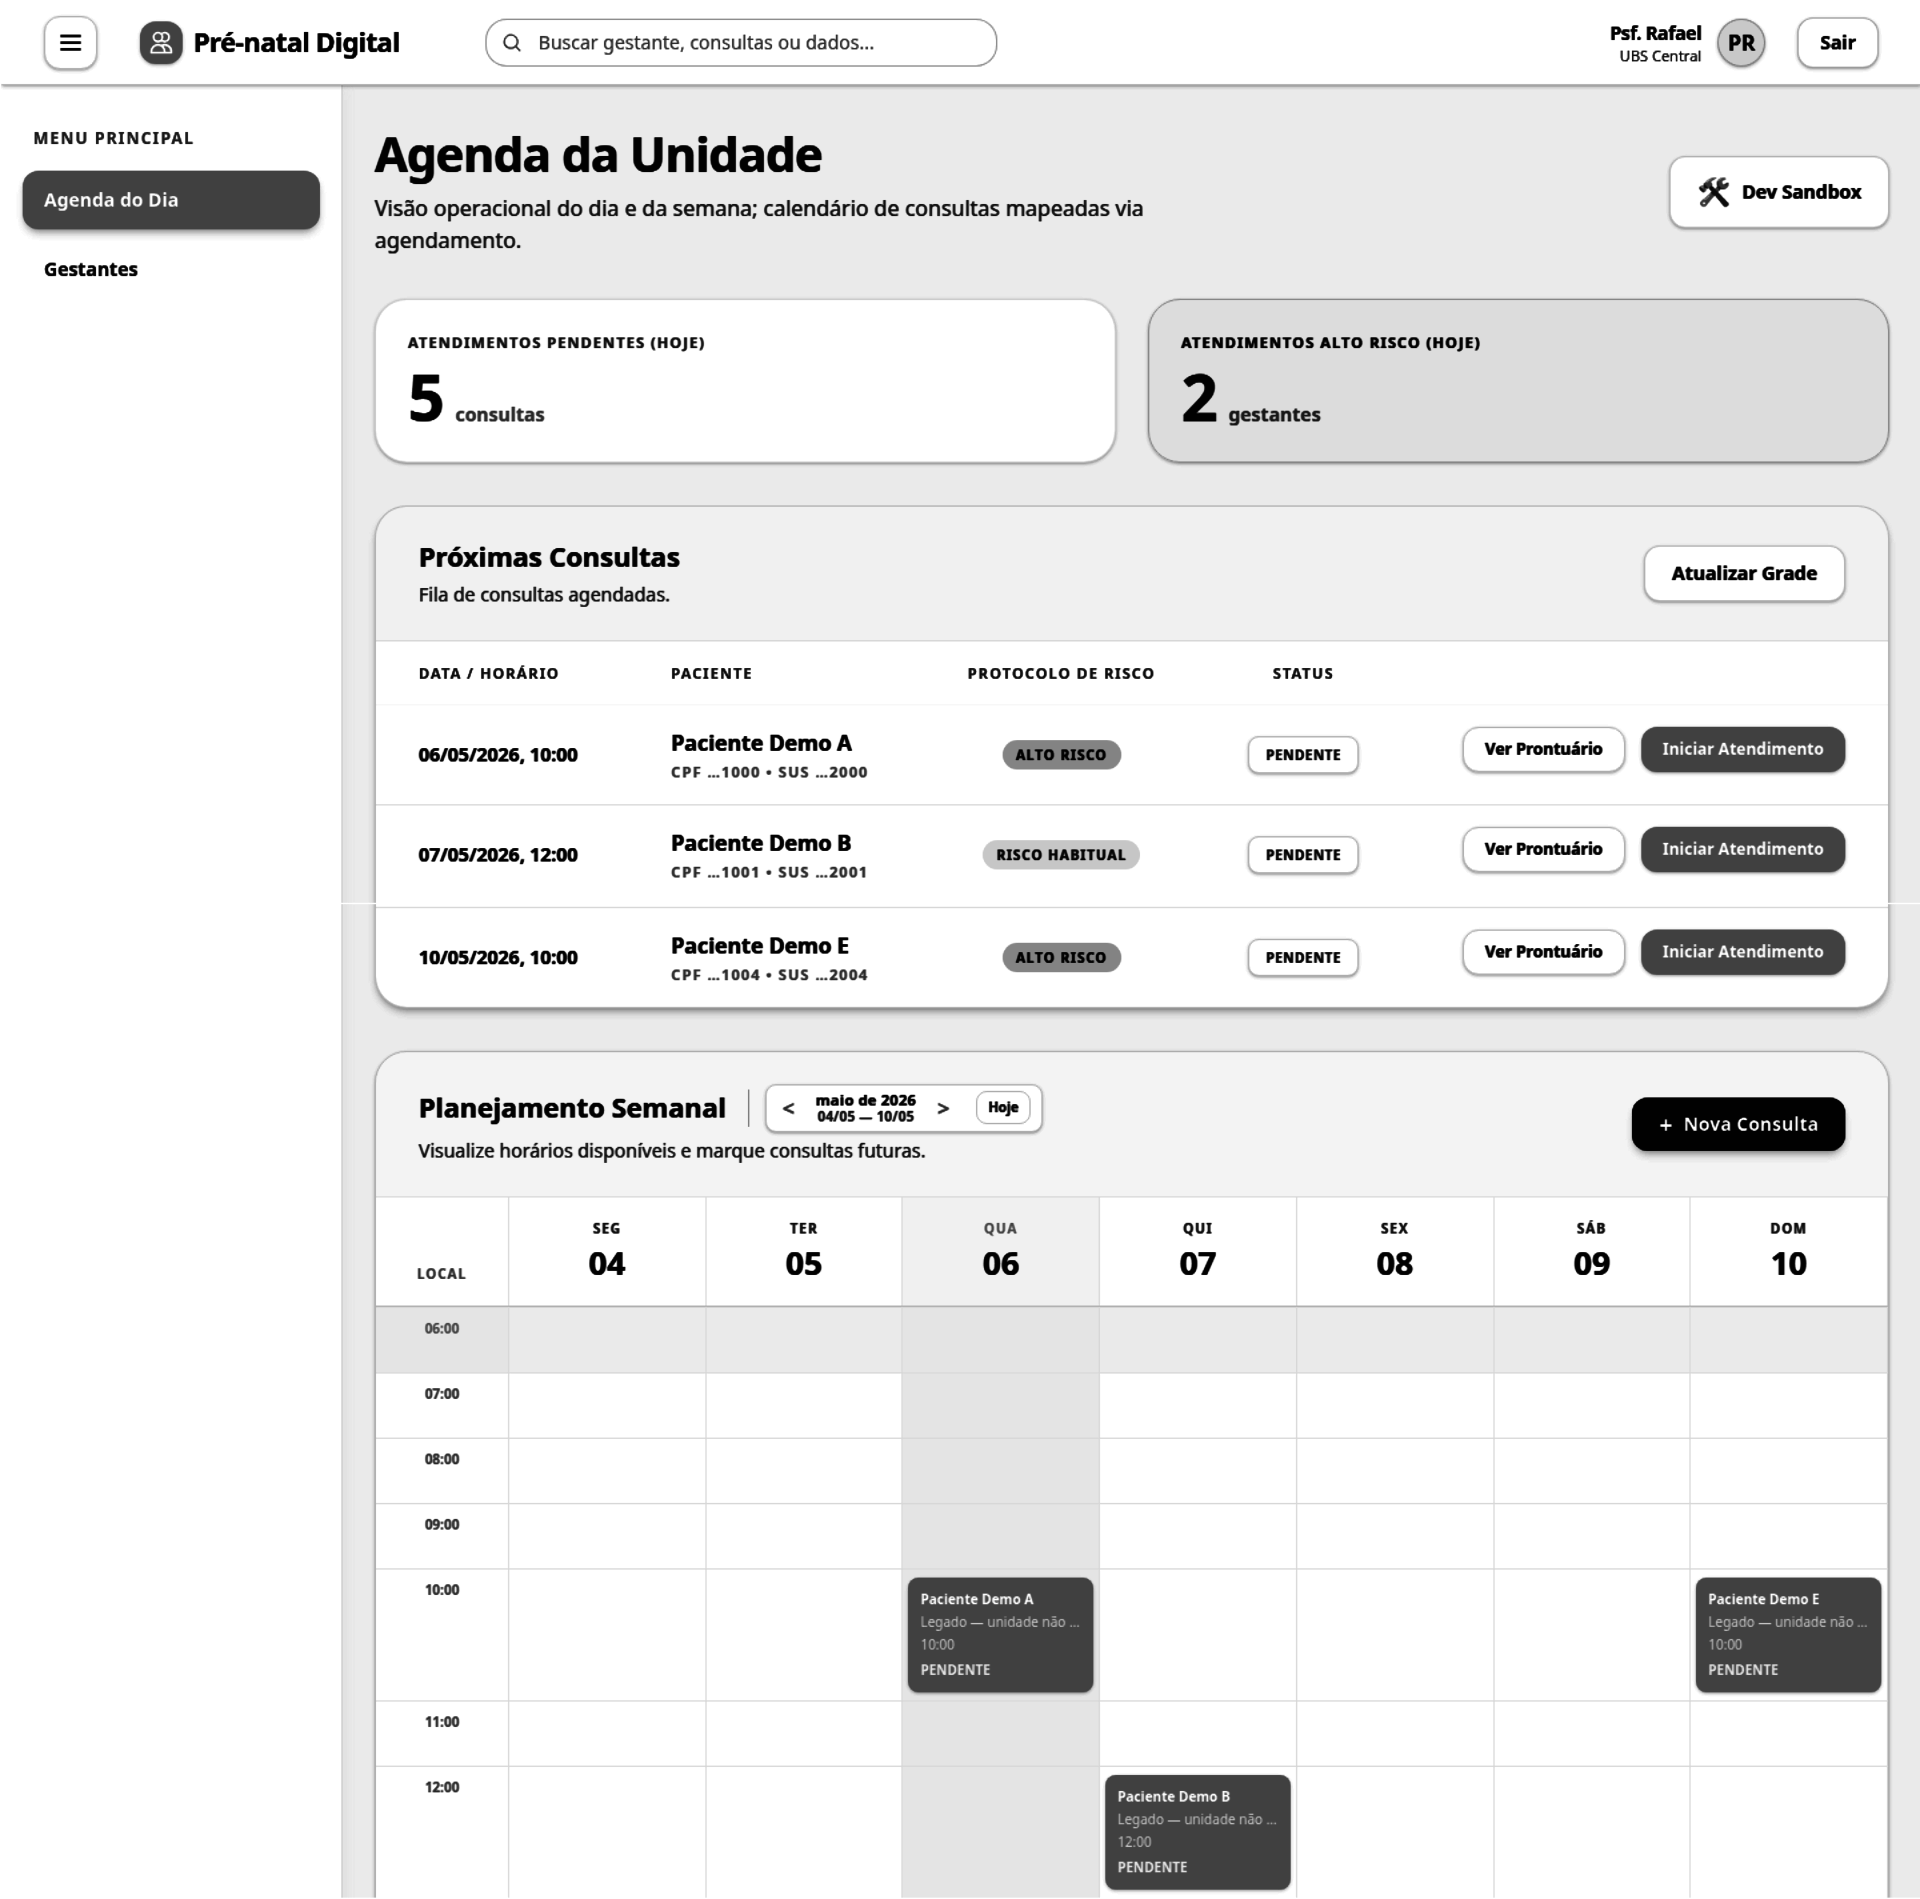
\includegraphics[width=\textwidth, trim={0 0 0 0}, clip]{assets/interfaces/alta_fidelidade/02_dashboard_editted_pb.png}
    \caption{Painel de gestão (Dashboard).}
    \label{fig:sub_dashboard}
  \end{subfigure}
  \hfill
  % --- Segunda Subfigura (Antiga Fig 4) ---
  \begin{subfigure}[b]{0.48\textwidth}
    \centering
    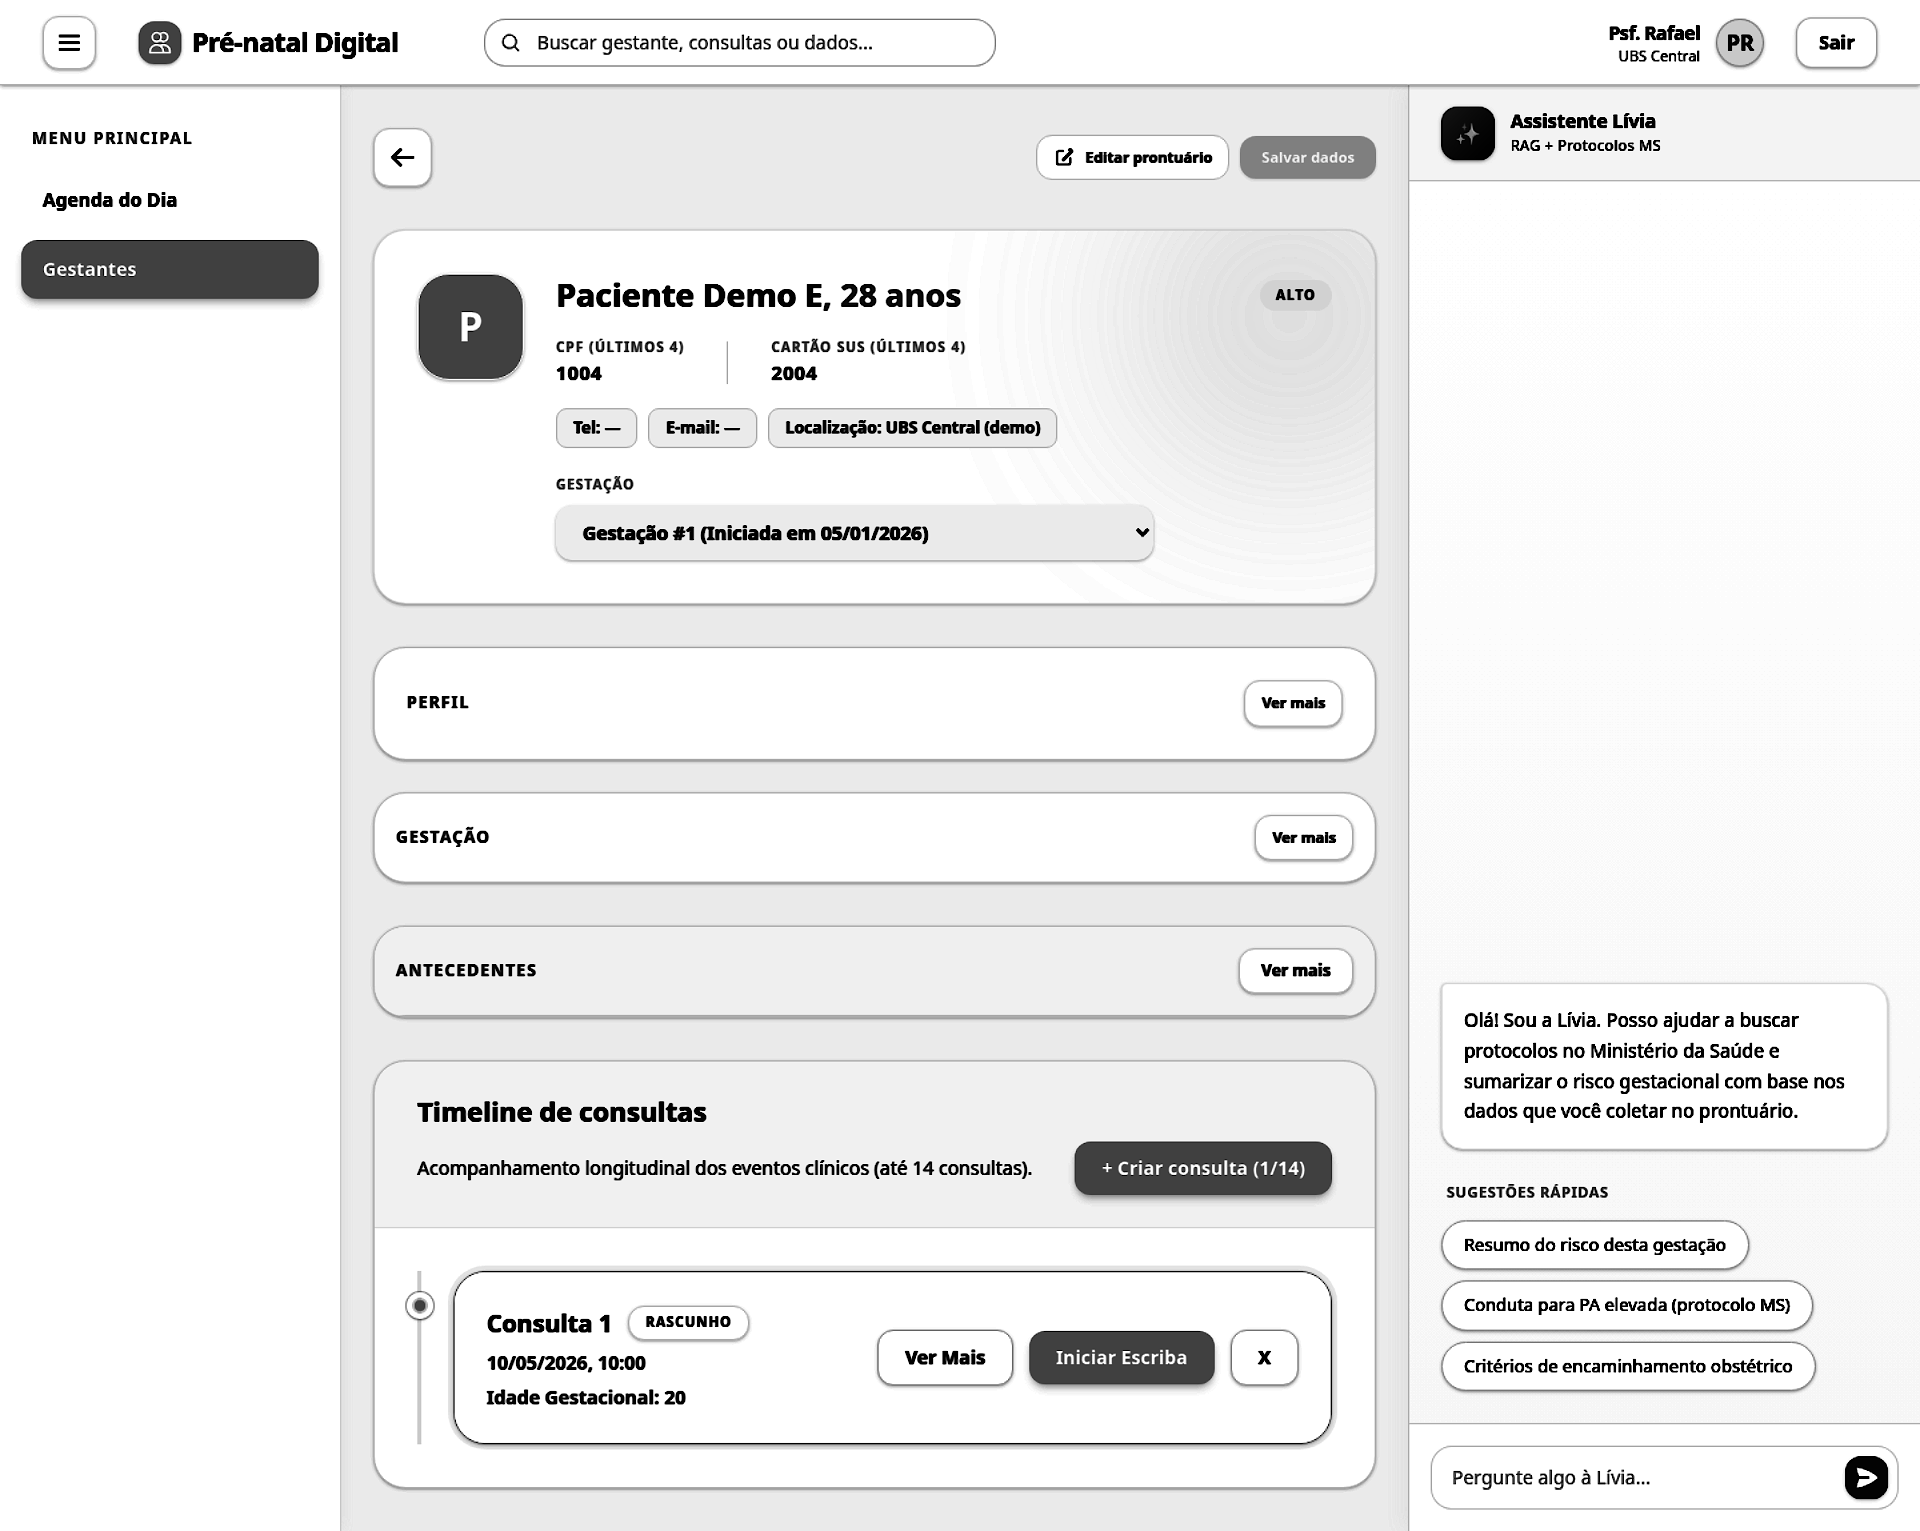
\includegraphics[width=\textwidth, trim={0 0 0 0}, clip]{assets/interfaces/alta_fidelidade/04_paciente_detalhe_pb.png}
    \caption{Visão consolidada do prontuário.}
    \label{fig:sub_paciente}
  \end{subfigure}

  \vspace{10pt} % Espaço entre as linhas de imagens

  % --- Terceira Subfigura (Antiga Fig 5) ---
  \begin{subfigure}[b]{0.9\textwidth}
    \centering
    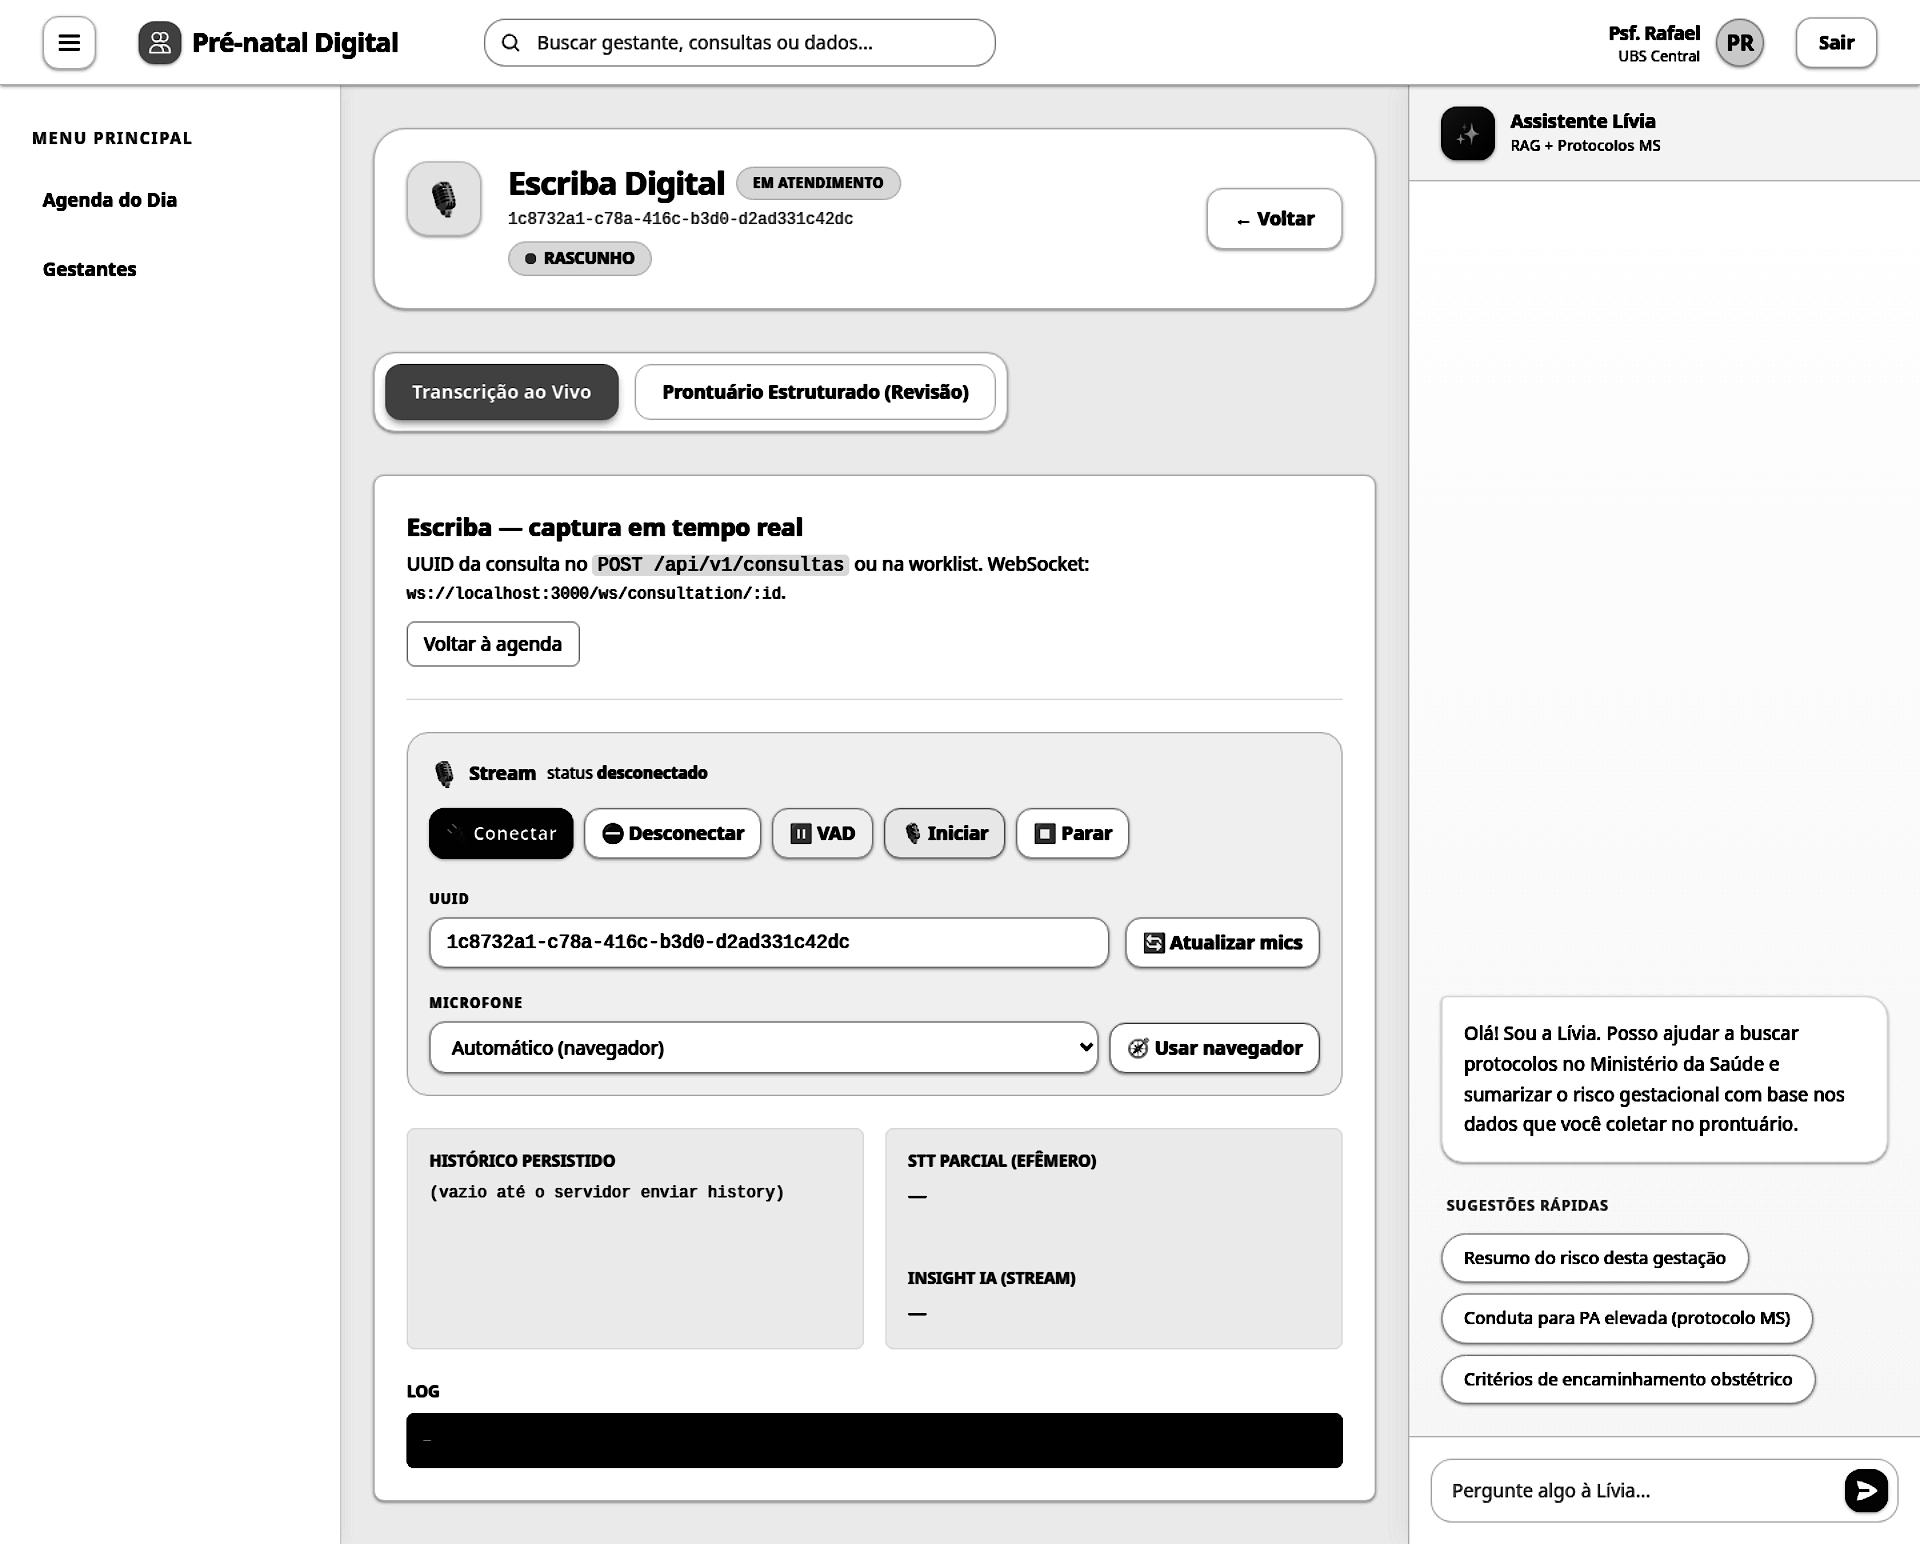
\includegraphics[width=\textwidth, trim={0 0 0 0}, clip]{assets/interfaces/alta_fidelidade/05_escriba_consulta_pb.png}
    \caption{Interface de atendimento em tempo real.}
    \label{fig:sub_escriba}
  \end{subfigure}

  \caption{Interfaces do protótipo de alta fidelidade: gestão, histórico e atendimento.}
  \label{fig:interfaces_compostas}
\end{figure}

Todo o código-fonte do ecossistema e suas respectivas configurações de \textit{deploy} foram disponibilizados em repositório público visando garantir a transparência e a reprodutibilidade do artefato construído \cite{Zegrine2026}.

%%%%%%%%%%%%%%%%%%%%%%%%%%%%%%%%%%%%%%%%%%%%%%%%%%%%%%%%%%%%%%%%%%%%%%%%%%%%%%%%%%%%%%%%%%%%%%%%%%%%%%%%%%%%%%%%%%%%%%%%%%%%%%%%%%%%%%%%%%%%%%%%%%%%%%%%%%%%%%%%%%%%%%

% Testes Executados + Resultados

\section{Avaliacao e Analise de Desempenho Do Pipelone RAG}

% Introducao da secao explicando que o RAG é avalido em duas etapas: Recuperacao e Geracao
Para garantir o rigor na avaliação do sistema proposto, o pipeline RAG foi submetido a uma bateria de testes utilizando um dataset de validação (Ground Truth).
Este conjunto contém perguntas reais de obstetrícia, formuladas sob a ótica de médicos e enfermeiros durante consultas de pré-natal, associadas às respostas exatas extraídas dos manuais do Ministério da Saúde.

\subsection{Avaliacao do moduilo de recuperacao de trechos semanticos (Retriever)}
% Consolidar as ideias sobre inferencia semantica e chunks
% Referencia: https://arxiv.org/abs/2309.15217
Nesta etapa, comprova-se a capacidade do banco de dados vetorial de retornar os trechos semânticos mais relevantes para a consulta da gestante.

\begin{itemize}
  \item \textbf{Accuracy/Hit@k}: Avalia a proporção de consultas em que pelo menos um documento relevante foi recuperado nos $k$ primeiros resultados.
  \begin{equation}
    Accuracy/Hit@k = \frac{TP + TN}{TP + TN + FP + FN}
  \end{equation}
  
  \item \textbf{Recall@k}: Mede a média harmônica entre a Precisão e o Recall, oferecendo uma métrica balanceada que penaliza tanto o excesso de falsos positivos (ruído no contexto) quanto falsos negativos (omissão de protocolo).
  \begin{equation}
    Recall@k = \frac{TP}{TP + FN}
  \end{equation}

  \item \textbf{F1-Score@k}: Combina precisão e recall, penalizando respostas excessivamente longas ou evasivas.
  \begin{equation}
    F1-Score@k = 2 * \frac{Precision@k * Recall@k}{Precision@k + Recall@k}
  \end{equation}
\end{itemize}

\subsection{Avaliacao do modulo de geracao de resposta (Generator)}
Com a disponibilidade dos trechos recuperados, avalia-se a capacidade do LLM de sintetizar a resposta clínica sem introduzir alucinações.

\begin{itemize}
  \item \textbf{Faithfulness}: Avalia se a resposta gerada pelo LLM foi baseada estritamente no contexto recuperado, penalizando severamente qualquer alucinação devido à criticidade dos protocolos de saúde.
  Em frameworks de avaliação modernos, pode ser calculada como a razão de sentenças factualmente suportadas pelo contexto:
  \begin{equation}
    Faithfulness = \frac{|V_{support}|}{|V_{total}|}
  \end{equation}
  Onde $V_{support}$ é o número de afirmações suportadas pelo contexto e $V_{total}$ é o total de afirmações na resposta.

  \item \textbf{Relevance}: Mede o quão direta e útil é a resposta para a pergunta clínica, penalizando saídas prolixas, evasivas ou incompletas.
  \begin{equation}
  \end{equation}
\end{itemize}

\section{Estudo Comparativo de Arquitetura: Modelos Locais vs. Nuvem}
% Aqui entra a sua ideia de provar que o modelo pequeno supera o grande usando RAG.
% Referencia: https://arxiv.org/abs/2309.15217
Para justificar as decisões de design arquitetural, especificamente a adoção de inferência local para preservação do sigilo médico, foi realizado um teste de benchmark comparativo.
O objetivo é comprovar empíricamente que um modelo local de menor escala, como o Qwen3.5 (9B), quando alimentado com os chunks semânticos corretos via RAG, obtém desempenho superior ou equivalente a modelos proprietários de larga escala operando em zero-shot sem contexto adicional (zero-shot).

\section{Efetividade Computacional e Latência}
Um sistema de suporte à decisão clínica não pode introduzir gargalos operacionais. O desempenho de infraestrutura foi monitorado através de:
\begin{itemize}
\item \textbf{Time To First Token (TTFT):} O tempo decorrido até a IA começar a gerar a resposta. Na prática clínica de médicos e enfermeiros, um TTFT superior a 2-3 segundos quebra o fluxo da consulta e inviabiliza a adoção.
\item \textbf{Latência de Recuperação (Retrieval Latency):} O tempo despendido exclusivamente na busca de similaridade no banco de dados vetorial, isolando a performance de I/O do tempo de inferência do LLM.
\end{itemize}

% \section{Avaliação Clínica e de Segurança (Expert Evaluation)}
% Além das métricas automatizadas, o agente IA foi submetido a casos clínicos simulados, avaliados sob o crivo de especialistas (médicos e enfermeiros).
% \begin{itemize}
% \item \textbf{Validação por Pares:} Um comitê de 3 a 5 profissionais de saúde avaliou uma amostra de 30 respostas do sistema utilizando uma escala Likert (1 a 5) nos critérios de \textit{Acurácia Científica} e \textit{Risco de Dano à Paciente}.
% \item \textbf{Taxa de Recusa Apropriada (Refusal Rate):} A porcentagem de vezes que o sistema, atuando sob as diretrizes de IA Responsável, recusou-se corretamente a responder perguntas que extrapolam o escopo dos manuais de pré-natal do Ministério da Saúde.
% \end{itemize}

% \section{Análise de Impacto na Carga Cognitiva}
% A premissa central da solução é mitigar a carga mental do profissional. O experimento foi conduzido dividindo profissionais em dois grupos de controle (ou cenários de teste cruzado):
% \begin{itemize}
% \item \textbf{Cenário A (Controle):} Profissionais estratificando o risco gestacional usando apenas a interface padrão do CRM e a consulta manual aos PDFs do Ministério da Saúde.
% \item \textbf{Cenário B (Proposto):} Profissionais realizando a mesma tarefa utilizando o CRM integrado ao agente IA.
% \end{itemize}
% A carga cognitiva foi medida comparativamente através do \textit{NASA Task Load Index (NASA-TLX)}, aliado ao tempo total de resolução do caso clínico.

%%%%%%%%%%%%%%%%%%%%%%%%%%%%%%%%%%%%%%%%%%%%%%%%%%%%%%%%%%%%%%%%%%%%%%%%%%%%%%%%%%%%%%%%%%%%%%%%%%%%%%%%%%%%%%%%%%%%%%%%%%%%%%%%%%%%%%%%%%%%%%%%%%%%%%%%%%%%%%%%%%%%%%

\section{Resultados}

% \subsection{Governança dos dados}
% Coleta das cartilhas de gestantes e guias para profissional de saude
% governanca e lgpd do banco de dados
% seguranca e anonimizadacao de dados enviados a IA
% human in the loop com aprovacoes da profissional da saude para os dados auto preenchidos pela IA
% mcp com tecnicas de seguranca para evitar vazamento de dados sensiveis via promp injection e sensitive data exposure

% \subsection{Auditoria de Equidade e Implementação de XAI}
% %<forte confirmacao medica dos dados preenchidos pela IA>
% O diferencial está na integração de técnicas de IA Explicável (XAI) e métricas de justiça (fairness) como requisitos de validação, e não somente como etapas pós-processamento.
% Para garantir que o modelo não perpetue preconceitos sistêmicos, serão aplicadas as métricas de Equalized Odds e Demographic Parity, comparando o erro residual entre diferentes grupos sociorraciais \cite{FairnessAI2023, ViesAlgoritmico2024}.

% Apresentacao dos trechos de chuinking que groundaram as respostas geradas pela IA
%   [GRÁFICO G1: Latência versus Nível de Quantização do Modelo Local]
%   [GRÁFICO G2: F1-Score do RAG em relação a diferentes tamanhos de janela de contexto recuperado.]
% Graficos de testes
% comparatrivos
% Espera-se um sistema replicavel com aumento significativo de interpretabilidade para profissionais de saúde, sem degradação estatisticamente relevante do desempenho em termos de Recall.
% A auditoria de equidade deverá evidenciar
% %<continuar>
% Espera-se também que a integração de técnicas de explicabilidade (XAI) contribua para maior confiança clínica no uso do sistema como apoio à decisão, reforçando seu potencial de adoção em ambientes reais do SUS.

%%%%%%%%%%%%%%%%%%%%%%%%%%%%%%%%%%%%%%%%%%%%%%%%%%%%%%%%%%%%%%%%%%%%%%%%%%%%%%%%%%%%%%%%%%%%%%%%%%%%%%%%%%%%%%%%%%%%%%%%%%%%%%%%%%%%%%%%%%%%%%%%%%%%%%%%%%%%%%%%%%%%%%

\section{Discussão}
% Retomada das perguntas norteadoras
% o resultado condiz com o que foi proposto? nao? porque?
% os resultados são generalizáveis? por que?
% quais os fatores limitantes encontrados?
% aumentar modelo x quantizar modelo custos e beneficios de cada um
%\subsection{Analise de custos e beneficios}
%    7.2 Analise de custos e beneficos
%     - Tradeoffs de privacidade vs usabilidade
%     - Tradeoffs de escalabilidade vs custo
%     - Testes realizados com o prototipo
%       - Testes de tolerancia a falhas - STT, RAG, LLM, Hardware, etc.
%       - Testes PII - nomes brasileiros complexos, girias regionasis, etc.
%         - Metrica: % de falso negativo na anonimizacao (grafico) % de dados que passaram para o llm sem a mascara aplicada
%     - Comparar latencia de um modelo de 7B rodando localmente vs a precisao para o contexto clinico (F1 score)
%       - F1 Score - Ground Truth - Criar 10 a 20 casos clinicos ficticios baseados na caderneta para servir de ground truth
% 8. Discussoes
%    - Limitacoes
%     - hardware e precos de implantacao real
%    - Riscos residuais de LLM
%    - Gestao de Riscos
%     - Prompt injection via MCP (mitigacao com context manager, readonly para o db, prompt shelding e sandboxing)
%     - STT latencia em hardware - faster whisper vs insanely fast whisper - diarizacao de audio vs transcricao de audio pura - sem diarizacao llm deve separar papeis em contexto
%     - RAG com recuperacao de chunks de ruido - reraking local top k
%     - STT nao robusto - fallback humano para validacao - stt so preenche dados
%    - Calibracao de confianca - sistema apresentar fontes de rag de forma explicita (citacao exata da caderneta) para o humano validar em segundos

% A implantação do sistema localmente apresenta fatores limitantes no que se refere aos recursos computacionais em postos de saúde, dada a necessidade de \textit{hardware} avançado (placas de vídeo com alta capacidade de memória VRAM ou Unidades de Processamento de Tensores) para viabilizar latências em tempo real tanto para a conversão áudio-texto quanto para as respostas do modelo generativo.


% Observa-se que a quantidade de contexto injetado no prompt através do processo RAG impõe desafios conhecidos como \textit{Lost in the Middle}, impactando diretamente o \textit{F1-Score} quando volumes extensivos de texto técnico são transferidos para o modelo de borda.

% talvez no futuro seja um sistema tao pesado 

% Finalmente, testes intensivos no módulo de Extração de Entidades Nomeadas (NER) e do protocolo MCP sinalizam que peculiaridades linguísticas (abreviações atípicas e coloquialismos) ainda representam pequenos riscos residuais para identificadores de saúde. Contudo, essa constatação suporta integralmente a necessidade da etapa metodológica adotada de \textit{human-in-the-loop}, que mitiga não apenas potenciais alucinações de conduta, mas valida a confiabilidade final da triagem registrada no banco de dados.

%%%%%%%%%%%%%%%%%%%%%%%%%%%%%%%%%%%%%%%%%%%%%%%%%%%%%%%%%%%%%%%%%%%%%%%%%%%%%%%%%%%%%%%%%%%%%%%%%%%%%%%%%%%%%%%%%%%%%%%%%%%%%%%%%%%%%%%%%%%%%%%%%%%%%%%%%%%%%%%%%%%%%%

\section{Conclusão}
% retomada dos atributos
% 9. Conclusão
%    - retomada dos objetivos e resultados
%    - Resumo dos Resultados
%      - Alinhamento com a cartilha da gestante SUS
%    - Contribuições
%    - Afimar viabilidade do projeto em locais de baixa conectividade, hardware limitado e alta privacidade
%    - Perspectivas (contribuicoes, viabilidade, proximos passos, trabalhos futuros)

% trbalho futuros com modelos moe ou pequenos com finetuning pe;os dados do ministerio para melhorar desempenho em hardwares de vram reduzida

% A arquitetura especificada no presente manuscrito consolida o design de um ecossistema digital \textit{on-premise} para o atendimento pré-natal no escopo do Sistema Único de Saúde, solucionando a premissa de que a LGPD restringe fluxos dependentes de processamento e extração remota em ambientes de nuvem pública. Por meio da combinação dos métodos \textit{Speech-to-Text} local, \textit{Retrieval-Augmented Generation} restrito às Cartilhas do Ministério da Saúde e do protocolo de anonimização estrito, atende-se ao objetivo de mitigar simultaneamente a elevada carga cognitiva e o risco de vazamento de dados.

% A viabilidade técnica comprova-se forte do ponto de vista do ciclo *software* e das blindagens de rede.

%%%%%%%%%%%%%%%%%%%%%%%%%%%%%%%%%%%%%%%%%%%%%%%%%%%%%%%%%%%%%%%%%%%%%%%%%%%%%%%%%%%%%%%%%%%%%%%%%%%%%%%%%%%%%%%%%%%%%%%%%%%%%%%%%%%%%%%%%%%%%%%%%%%%%%%%%%%%%%%%%%%%%%

% 10. Referências
%     - Bibliografia
%     - Links de interesse

\newpage

\bibliographystyle{sbc}
\bibliography{sbc-template}

\end{document}
